%%%%%%%%%%%%%%%%%%%%%%%%%%%%%%%%%%%%%%%%%
% Beamer Presentation
% LaTeX Template
% Version 1.0 (10/11/12)
%
% This template has been downloaded from:
% http://www.LaTeXTemplates.com
%
% License:
% CC BY-NC-SA 3.0 (http://creativecommons.org/licenses/by-nc-sa/3.0/)
%
%%%%%%%%%%%%%%%%%%%%%%%%%%%%%%%%%%%%%%%%%

%----------------------------------------------------------------------------------------
%	PACKAGES AND THEMES
%----------------------------------------------------------------------------------------

\documentclass{beamer}

\mode<presentation> {

% The Beamer class comes with a number of default slide themes
% which change the colors and layouts of slides. Below this is a list
% of all the themes, uncomment each in turn to see what they look like.

%\usetheme{default}
%\usetheme{AnnArbor}
%\usetheme{Antibes}
%\usetheme{Bergen}
%\usetheme{Berkeley}
%\usetheme{Berlin}
%\usetheme{Boadilla}
%\usetheme{CambridgeUS}
%\usetheme{Copenhagen}
%\usetheme{Darmstadt}
%\usetheme{Dresden}
%\usetheme{Frankfurt}
%\usetheme{Goettingen}
%\usetheme{Hannover}
%\usetheme{Ilmenau}
%\usetheme{JuanLesPins}
%\usetheme{Luebeck}
\usetheme{Madrid}
%\usetheme{Malmoe}
%\usetheme{Marburg}
%\usetheme{Montpellier}
%\usetheme{PaloAlto}
%\usetheme{Pittsburgh}
%\usetheme{Rochester}
%\usetheme{Singapore}
%\usetheme{Szeged}
%\usetheme{Warsaw}

% As well as themes, the Beamer class has a number of color themes
% for any slide theme. Uncomment each of these in turn to see how it
% changes the colors of your current slide theme.

%\usecolortheme{albatross}
%\usecolortheme{beaver}
%\usecolortheme{beetle}
%\usecolortheme{crane}
%\usecolortheme{dolphin}
%\usecolortheme{dove}
%\usecolortheme{fly}
%\usecolortheme{lily}
%\usecolortheme{orchid}
%\usecolortheme{rose}
%\usecolortheme{seagull}
%\usecolortheme{seahorse}
%\usecolortheme{whale}
%\usecolortheme{wolverine}

\setbeamertemplate{footline}{} % To remove the footer line in all slides uncomment this line
\setbeamertemplate{footline}[page number] % To replace the footer line in all slides with a simple slide count uncomment this line

\setbeamertemplate{navigation symbols}{} % To remove the navigation symbols from the bottom of all slides uncomment this line
}

\usepackage{graphicx} % Allows including images
\usepackage{booktabs} % Allows the use of \toprule, \midrule and \bottomrule in tables
%\usepackage {tikz}
\usepackage{tkz-graph}
\usepackage{bbm}
\GraphInit[vstyle = Shade]
\tikzset{
  LabelStyle/.style = { rectangle, rounded corners, draw,
                        minimum width = 2em, fill = yellow!50,
                        text = red, font = \bfseries },
  VertexStyle/.append style = { inner sep=5pt,
                                font = \normalsize\bfseries},
  EdgeStyle/.append style = {->, bend left} }
\usetikzlibrary {positioning}
%\usepackage {xcolor}
\definecolor {processblue}{cmyk}{0.96,0,0,0}
%----------------------------------------------------------------------------------------
%	TITLE PAGE
%----------------------------------------------------------------------------------------

\title[Short title]{Introduction to Sequential minimal optimization} % The short title appears at the bottom of every slide, the full title is only on the title page

\author{Yinbin Ma} % Your name
\institute[UC Riverside] % Your institution as it will appear on the bottom of every slide, may be shorthand to save space
{
University of Illinois at Chicago \\ % Your institution for the title page
\medskip
}
\date{\today} % Date, can be changed to a custom date

\begin{document}

\begin{frame}
\titlepage % Print the title page as the first slide
\end{frame}

\begin{frame}
\frametitle{Overview} % Table of contents slide, comment this block out to remove it
\tableofcontents % Throughout your presentation, if you choose to use \section{} and \subsection{} commands, these will automatically be printed on this slide as an overview of your presentation
\end{frame}

%----------------------------------------------------------------------------------------
%	PRESENTATION SLIDES
%----------------------------------------------------------------------------------------

%------------------------------------------------

\section{Objective function of SVM}
\begin{frame}{Introduction}
Support Vector Machine aims to find a decision boundary with maximum margin. Lets $ X \in \mathbb{R}^{N\times K}, y \in \mathbb{R}^N, y_i \in \{-1, 1\}, w \in \mathbb{R}^K, b \in \mathbb{R}$. The objective function is:
\begin{gather*}
\min_{w, b, \xi} \quad \frac{1}{2}||w||^2 + C \sum_{i=1}^N{\xi_i} \\
s.t. \quad y_i(w^T x_i + b) \geq 1 - \xi_i \quad \xi_i \geq 0
\end{gather*}
\end{frame}

\section{Convex Optimizing}
\begin{frame}{Lagrangian}

To Solve it and find the optimal result, we start by defining the generalized Lagrangian.

\begin{align*}
\mathcal{L}(w, b, \xi, \alpha, \beta) &= \frac{1}{2}w^T w+C\sum_i^N{\xi_i} \\ &-\sum_i^N{\alpha_i \biggl( y_i (w^T x_i + b) - 1 + \xi_i \biggr)} - \sum_i^N{\beta_i \xi_i} \\
s.t. &\quad \alpha_i \geq 0 \quad \beta_i \geq 0
\end{align*}
\end{frame}

\begin{frame}{Primal Problem}
Lets say $\theta_{p}(w) = \max_{\alpha,\beta: \alpha_i \geq 0} \mathcal{L} (w, b, \xi, \alpha, \beta)$, if $w$ is given but it violates any of the constraints, we will have $\theta_{p}(w) \rightarrow \infty $. Hence 
\begin{gather*}
\theta_{p}(w) = 
\begin{cases}
\frac{1}{2}w^T w \quad &\text{if w satisfies constraints} \\
\infty \quad &\text{otherwise}
\end{cases}
\end{gather*}
Then we $\min_w{\theta_{p}(w)} = \min_w{\max_{\alpha,\beta: \alpha_i \geq 0} \mathcal{L}(w, b, \xi, \alpha, \beta)} $, and we get a qualified $w$.
However $\theta_{p}(w)$ is trivial. 
\end{frame}

\begin{frame}{Dual Problem}
Supposing we have $\theta_d(\alpha, \beta) = \min_{w}\mathcal{L}(w, b, \xi, \alpha, \beta)$, and it is shown that 

$$
d^* = \max_{\alpha,\beta: \alpha_i \geq 0} \theta_d(\alpha, \beta) \leq \min_w{\theta_{p}(w)} = p^*
$$

Under certain conditions, we could have $d^* = p^*$, so we could solve dual problem instead of primal problem. The conditions are called \textbf{Karush-Kuhn-Tucker (KKT) conditions}.
\end{frame}

\begin{frame}{Karush-Kuhn-Tucker Conditions}
Consider the following, which we’ll call the primal optimization problem:
\begin{align*}
    \min_{w} \quad &f(w) \\
    s.t. \quad &g_i(w) \leq 0, i = 1, \dots ,k \\
    &h_i(w) = 0, i = 1, \dots , p
\end{align*}
Suppose $f$ and each $g_i$ are convex, and each $h_i$ is affine which means linear. Suppose further that there exists some $w$ so that $g_i(w) < 0$ for all $i$. \\
\end{frame}

\begin{frame}{Karush-Kuhn-Tucker Conditions}
The corresponding Lagrangian is 
\begin{gather*}
    \mathcal{L}(w, \alpha, \beta) = f(w) + \sum_{i=1}^k{\alpha_i g_i(w)} + \sum_{i=1}^p{\beta_i h_i(w)}
\end{gather*}
Under above assumptions, there must exists $w^*, \alpha^*, \beta^*$, so that $w^*$ is the solution to the primal problem, $\alpha^*, \beta^*$ are the solution to the dual problem, and moreover $p^* = d^* = \mathcal{L}(w^*, \alpha^*, \beta^*)$. Further more, we have:
\begin{align}
    \bigtriangledown_{w_i}\mathcal{L}(w^*, \alpha^*, \beta^*) &= 0 \\
    \bigtriangledown_{\beta_i}\mathcal{L}(w^*, \alpha^*, \beta^*) &= 0 \\
    \alpha^*_i g_i(w^*) &= 0 \\
    g_i(w^*) &\leq 0 \\
    \alpha^* &\geq 0
\end{align}
\end{frame}

\begin{frame}{Optimizing}
\begin{align*}
\mathcal{L}(w, b, \xi, \alpha, \beta) &= \frac{1}{2}w^T w+C\sum_i^N{\xi_i} \\ &-\sum_i^N{\alpha_i \biggl( y_i (w^T x_i + b) - 1 + \xi_i \biggr)} - \sum_i^N{\beta_i \xi_i} \\
s.t. &\quad \alpha_i \geq 0 \quad \beta_i \geq 0
\end{align*}
Lets take some derivatives:
\begin{align*}
\bigtriangledown_w\mathcal{L}(w, b, \xi, \alpha, \beta) &= w - \sum_{i=1}^N{\alpha_i y_i x_i} = 0 \\
\bigtriangledown_b\mathcal{L}(w, b, \xi, \alpha, \beta) &= -\sum_{i=1}^N{\alpha_i y_i} = 0 \\
\bigtriangledown_{\xi_i}\mathcal{L}(w, b, \xi, \alpha, \beta) &= C - \alpha_i - \beta_i = 0
\end{align*}
\end{frame}

\begin{frame}{Optimizing}
So we know that
\begin{gather*}
    w = \sum_{i=1}^N{\alpha_i y_i x_i} \quad
    \sum_{i=1}^N{\alpha_i y_i} = 0 \quad
    C - \alpha_i - \beta_i = 0
\end{gather*}
Take these equations and plug them back into the Lagrangian, and simplify. Then we obtain the following dual optimization problem:
\begin{align*}
    \min_\alpha \quad \frac{1}{2} &\sum_{i=1}^N \sum_{j=1}^N \alpha_i \alpha_j y_i y_j \bigl< x_i,x_j \bigr> - \sum_{i=1}^N \alpha_i \\
    s.t. \quad & \sum_{i=1}^N \alpha_i y_i = 0 \\
    & 0 \leq \alpha_i \leq C
\end{align*}
\end{frame}

\begin{frame}{Optimizing}
\begin{align*}
    \min_\alpha \quad \frac{1}{2} &\sum_{i=1}^N \sum_{j=1}^N \alpha_i \alpha_j y_i y_j\bigl< x_i,x_j \bigr> - \sum_{i=1}^N \alpha_i \\
    s.t. \quad & \sum_{i=1}^N \alpha_i y_i = 0 \\
    & 0 \leq \alpha_i \leq C
\end{align*}
After we obtain a satisfied $\alpha$, we could construct a classifier:
\begin{gather*}
    f(x) = sign(\sum_{i=1}^N \alpha_i y_i \bigl< x_i,x \bigr> + b)
\end{gather*}
\end{frame}

\begin{frame}{Optimizing}
Due to \textbf{KKT conditions} and further lemmas, we know that:
\begin{gather*}
    \alpha_i \bigl( y_i (w^T x_i + b) - 1 + \xi_i \bigr) = 0 \quad \beta_i \xi_i = 0 \\
    y_i(w^T x_i + b - 1 + \xi_i) \geq 0 \quad C - \beta_i - \alpha_i = 0
\end{gather*}

If a $x_i, y_i$ pair satisfied constraints, it will follow:
\begin{alignat*}{4}
 \alpha_i = 0 &\Rightarrow& \beta_i = C &, \xi_i=0 &\Rightarrow y_i(w^T x_i + b) \geq 1 \\ 
 0 < \alpha_i < C &\Rightarrow& 0 < \beta_i < C &, \xi_i = 0 &\Rightarrow y_i(w^T x_i + b) = 1 \\  
 \alpha_i = C &\Rightarrow &\beta_i = 0 &, \xi_i \geq 0 &\Rightarrow y_i(w^T x_i + b) \leq 1    
\end{alignat*}

In next slide, we will utilize this lemma to test if final result is converged.
\end{frame}

\section{SMO Algorithm}
\begin{frame}{What's SMO?}
    Sequential minimal optimization (SMO) is an algorithm for solving the quadratic programming (QP) problem that arises during the training of SVM. It was invented by John Platt in 1998 at Microsoft Research. In SVM, the QP problem is expressed as follow:
    \begin{align}
        \min_\alpha \quad \frac{1}{2} &\sum_{i=1}^N \sum_{j=1}^N \alpha_i \alpha_j y_i y_j\bigl< x_i,x_j \bigr> - \sum_{i=1}^N \alpha_i \\
        s.t. \quad & \sum_{i=1}^N \alpha_i y_i = 0 \\
        & 0 \leq \alpha_i \leq C
    \end{align}
\end{frame}

\begin{frame}{What's SMO?}
    In constraint (7), lets say we select $\alpha_1, \alpha_2$ from $\alpha$, then fix the rest of variables, which means treating them as a constant, then we could have:
    \begin{gather*}
        \alpha_1 y_1 + \alpha_2 y_2 = - \sum_{i=3}^N \alpha_i y_i = \zeta
    \end{gather*}
    So the QP problem seperate several subproblems, we assume $K = X X^T \in \mathbb{R}^{N \times N}$, and one of subproblems is shown as follow:
    \begin{align*}
        \min_{\alpha_1, \alpha_2} \ W(\alpha_1, \alpha_2) &= \frac{1}{2}K_{11} {\alpha_1}^2 + \frac{1}{2} K_{22} {\alpha_2}^2 + y_1 y_2 K_{12} \alpha_1 \alpha_2 \\  &- (\alpha_1 + \alpha_2) + y_1 \alpha_1 \sum_{i=3}^{N}{y_i \alpha_i K_{i1}} + y_2 \alpha_2 \sum_{i=3}^{N}{y_i \alpha_i K_{i2}} \\
        s.t. \ &\alpha_1 y_1 + \alpha_2 y_2 = \zeta \qquad
        0 \leq \alpha_1 \leq C, \ i = 1,2 
    \end{align*}
\end{frame}

\begin{frame}{Subproblem Optimizing}
    Due to the constraint, $\alpha_1, \alpha_2$ must lie within the box $[0, C] \times [0, C]$ as shown below:
    \begin{figure}
    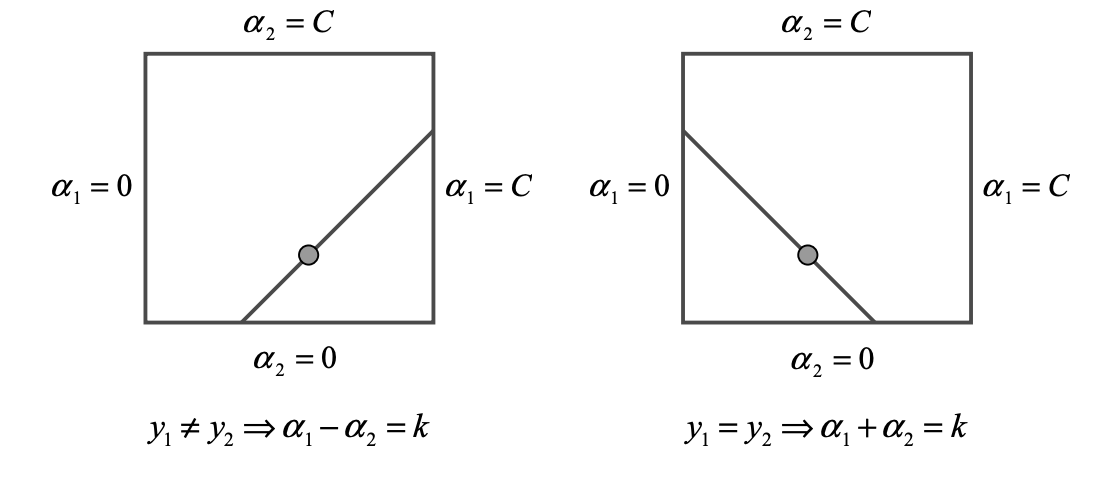
\includegraphics[width=120mm]{alpha.png}
    \end{figure}
\end{frame}

\begin{frame}{Subproblem Optimizing}
    The following bounds apply to $\alpha_2 \in [L, H]$ is:
    \begin{gather*}
        L = 
        \begin{cases}
            \max(0, \alpha_2 + \alpha_1 - C) & y_1 = y_2 \\
            \max(0, \alpha_2 - \alpha_1) & y_1 \neq y_2
        \end{cases}
        \\
        H = \begin{cases}
            \min(C, \alpha_2 + \alpha_1) & y_1 = y_2 \\
            \min(C, \alpha_2 - \alpha_1 + C) & y_1 \neq y_2
        \end{cases}
    \end{gather*}
\end{frame}

\begin{frame}{Subproblem Optimizing}
    Lets say:
    \begin{gather*}
        E_i = \sum_{j=1}^N \alpha_i y_i \bigl< x_i, x_j \bigr> + b - y_i \\
        \eta = K_{11} + K_{22} - 2K_{12} \\
        \alpha_2^{unclip} = \alpha_2 + \frac{y_2(E_1 - E_2)}{\eta}
     \end{gather*}
     The result need to be clipped:
     \begin{gather*}
        \alpha_2^{new} = \begin{cases}
        H &\text{if } \alpha_2^{unclip} > H \\
        L &\text{if } \alpha_2^{unclip} < L \\
        \alpha_2^{unclip} &\text{otherwise}
        \end{cases}
     \end{gather*}
     After we obtain the $\alpha_2$, we could get $\alpha_1^{new} = \alpha_1^{old} + y_1y_2\bigl(\alpha_2^{old} - \alpha_2^{new}\bigr)$.
\end{frame}

\begin{frame}{Update other variables}
    For next iteration, we need to update $b$ and $E_i$, For $j \in \{1, 2\}$.
    \begin{gather*}
        \because \sum_{i=1}^N \alpha_i y_i K_{ij} + b_j = y_j \\
        \therefore b_j^{new} = y_j - \sum_{i=3}^N \alpha_i y_i K_{ij} - \alpha_1^{new} K_{1j} - \alpha_2^{new} K_{2j} \\
        b^{new} = \begin{cases}
        b_1^{new}, &\text{if } \alpha_1 \in (0, C) \\
        b_2^{new}, &\text{if } \alpha_2 \in (0, C) \\
        (b_1^{new}+b_2^{new})/2, &\text{otherwise}
        \end{cases} \\
        E_j^{new} = \sum_{i \in S} y_i \alpha_i K_{ij} + b^{new} - y_i
    \end{gather*}
    $S$ is the set of support vectors, which means $y_i(w^Tx_i + b) \leq 1$.
\end{frame}

\begin{frame}{Select $\alpha_1$ and $\alpha_2$}
    In most of full SMO algorithm implements, they are dedicated to heuristics to maximize the objective function as much as possible. \\ 
    However, in practical we follow a simplified version. First we iterate $\alpha_i$ and check if it violates KKT conditions, then we select it as $\alpha_2$ and we randomly choose $\alpha_1$ from the remaining $\alpha_i$ and attempt to jointly optimize $\alpha_1, \alpha_2$. \\
    Repeat this step on all $\alpha_i$, and check if all $\alpha_i$ are obey the KKT conditions. If they are, we could yield the $\alpha$, and construct the classifier:
    \begin{gather*}
        f(x) = sign(\sum_{i \in S} \alpha_i y_i \bigl< x_i,x \bigr> + b) \\
        S = \{\alpha_i | \alpha_i \in \alpha, \alpha_i \neq 0\}
    \end{gather*}
\end{frame}

\section{Other Optimizing Algorithm}
\begin{frame}{Gradient Optimization}
    In general, the primal problem could be written as:
    \begin{gather*}
        \min_{w, b} \quad \mathcal{L}(w, b) = \sum_{i=1}^N \mathbbm{1}\biggl[ 1 - y_i \bigl( w \cdot x_i + b\bigr) \biggr] + \lambda || w ||^2
    \end{gather*}
    Just take the derivatives:
    \begin{align*}
        \bigtriangledown_{w} \mathcal{L}(w, b) &= - \sum_{i=1}^N \mathbbm{1}\biggl[ 1 - y_i\bigl(w \cdot x_i + b\bigr) \biggr] y_i x_i + 2 \lambda w \\
        \bigtriangledown_{b} \mathcal{L}(w, b) &= - \sum_{i=1}^N \mathbbm{1}\biggl[ 1 - y_i\bigl(w \cdot x_i + b\bigr) \biggr] y_i
    \end{align*}
    Therefore, we first initialize $w, b$, and set the learning rate $\eta$. Using the gradient optimization, the $\mathcal{L}(w, b)$ will converge at a minimal point.  
\end{frame}

\section{Reference}
    \begin{frame}{Reference}
    Stanford CS229 class notes and section notes.
    \begin{itemize}
        \item \href{http://cs229.stanford.edu/materials/smo.pdf}{Autumn 2009
        The Simplified SMO Algorithm.}
        \item \href{http://cs229.stanford.edu/notes-spring2019/cs229-notes3.pdf}{Lecture Notes 3, Andrew Ng.}
    \end{itemize}
    Paper
    \begin{itemize}
        \item \href{https://www.microsoft.com/en-us/research/wp-content/uploads/2016/02/tr-98-14.pdf}{Platt, J. (1998). Sequential minimal optimization: A fast algorithm for training support vector machines.}
        \item \href{https://www.csie.ntu.edu.tw/~cjlin/papers/libsvm.pdf}{C.-C. Chang and C.-J. Lin. LIBSVM : a library for support vector machines. ACM Transactions on Intelligent Systems and Technology, 2:27:1--27:27, 2011.}
    \end{itemize}
\end{frame}

\begin{frame}
    \Huge{\centerline{The End}}
\end{frame}

\end{document}
